\subsection{\href{https://www.lacolmena.com.ar/}{La Colmena}}
   \hypertarget{subsec:colmena}
   Para la conocida disco de Pilar, La Colmena, se desarrolló y fabricó un techo de leds controlado por ethernet con el sofisticado software alemán Madrix, de destacan las fotos de la instalación en la figura \ref{fig:colmena} y tambien estan publicados algunos \href \linkcolmenavideos {videos}.
   \begin{figure}
      \begin{center}
         \includegraphics[width=0.24\textwidth]{colmena1.jpg}
         \includegraphics[width=0.24\textwidth]{colmena2.jpg}
         \includegraphics[width=0.24\textwidth]{colmena3.jpg}
         \includegraphics[width=0.24\textwidth]{colmena4.jpg}
      \end{center}
      \caption{Pantalla de leds montada en el techo de la disco La Colmena, desarrollada, fabricada e instalada}
      \label{fig:colmena}
   \end{figure}
   \par
   De este trabajo se desprendió un producto que consiste en módulos interconectarles para formar pantallas de leds de diferentes pitch y tamanos. Se pueden apreciar en las fotos de la figura \ref{fig:ledcover} y se pueden ver algunos videos en \href \linkledcovervideos {videos}.
   \begin{figure}
      \begin{center}
         \includegraphics[width=0.24\textwidth]{ledcover1.jpg}
         \includegraphics[width=0.24\textwidth]{ledcover2.jpg}
         \includegraphics[width=0.24\textwidth]{ledcover3.jpg}
         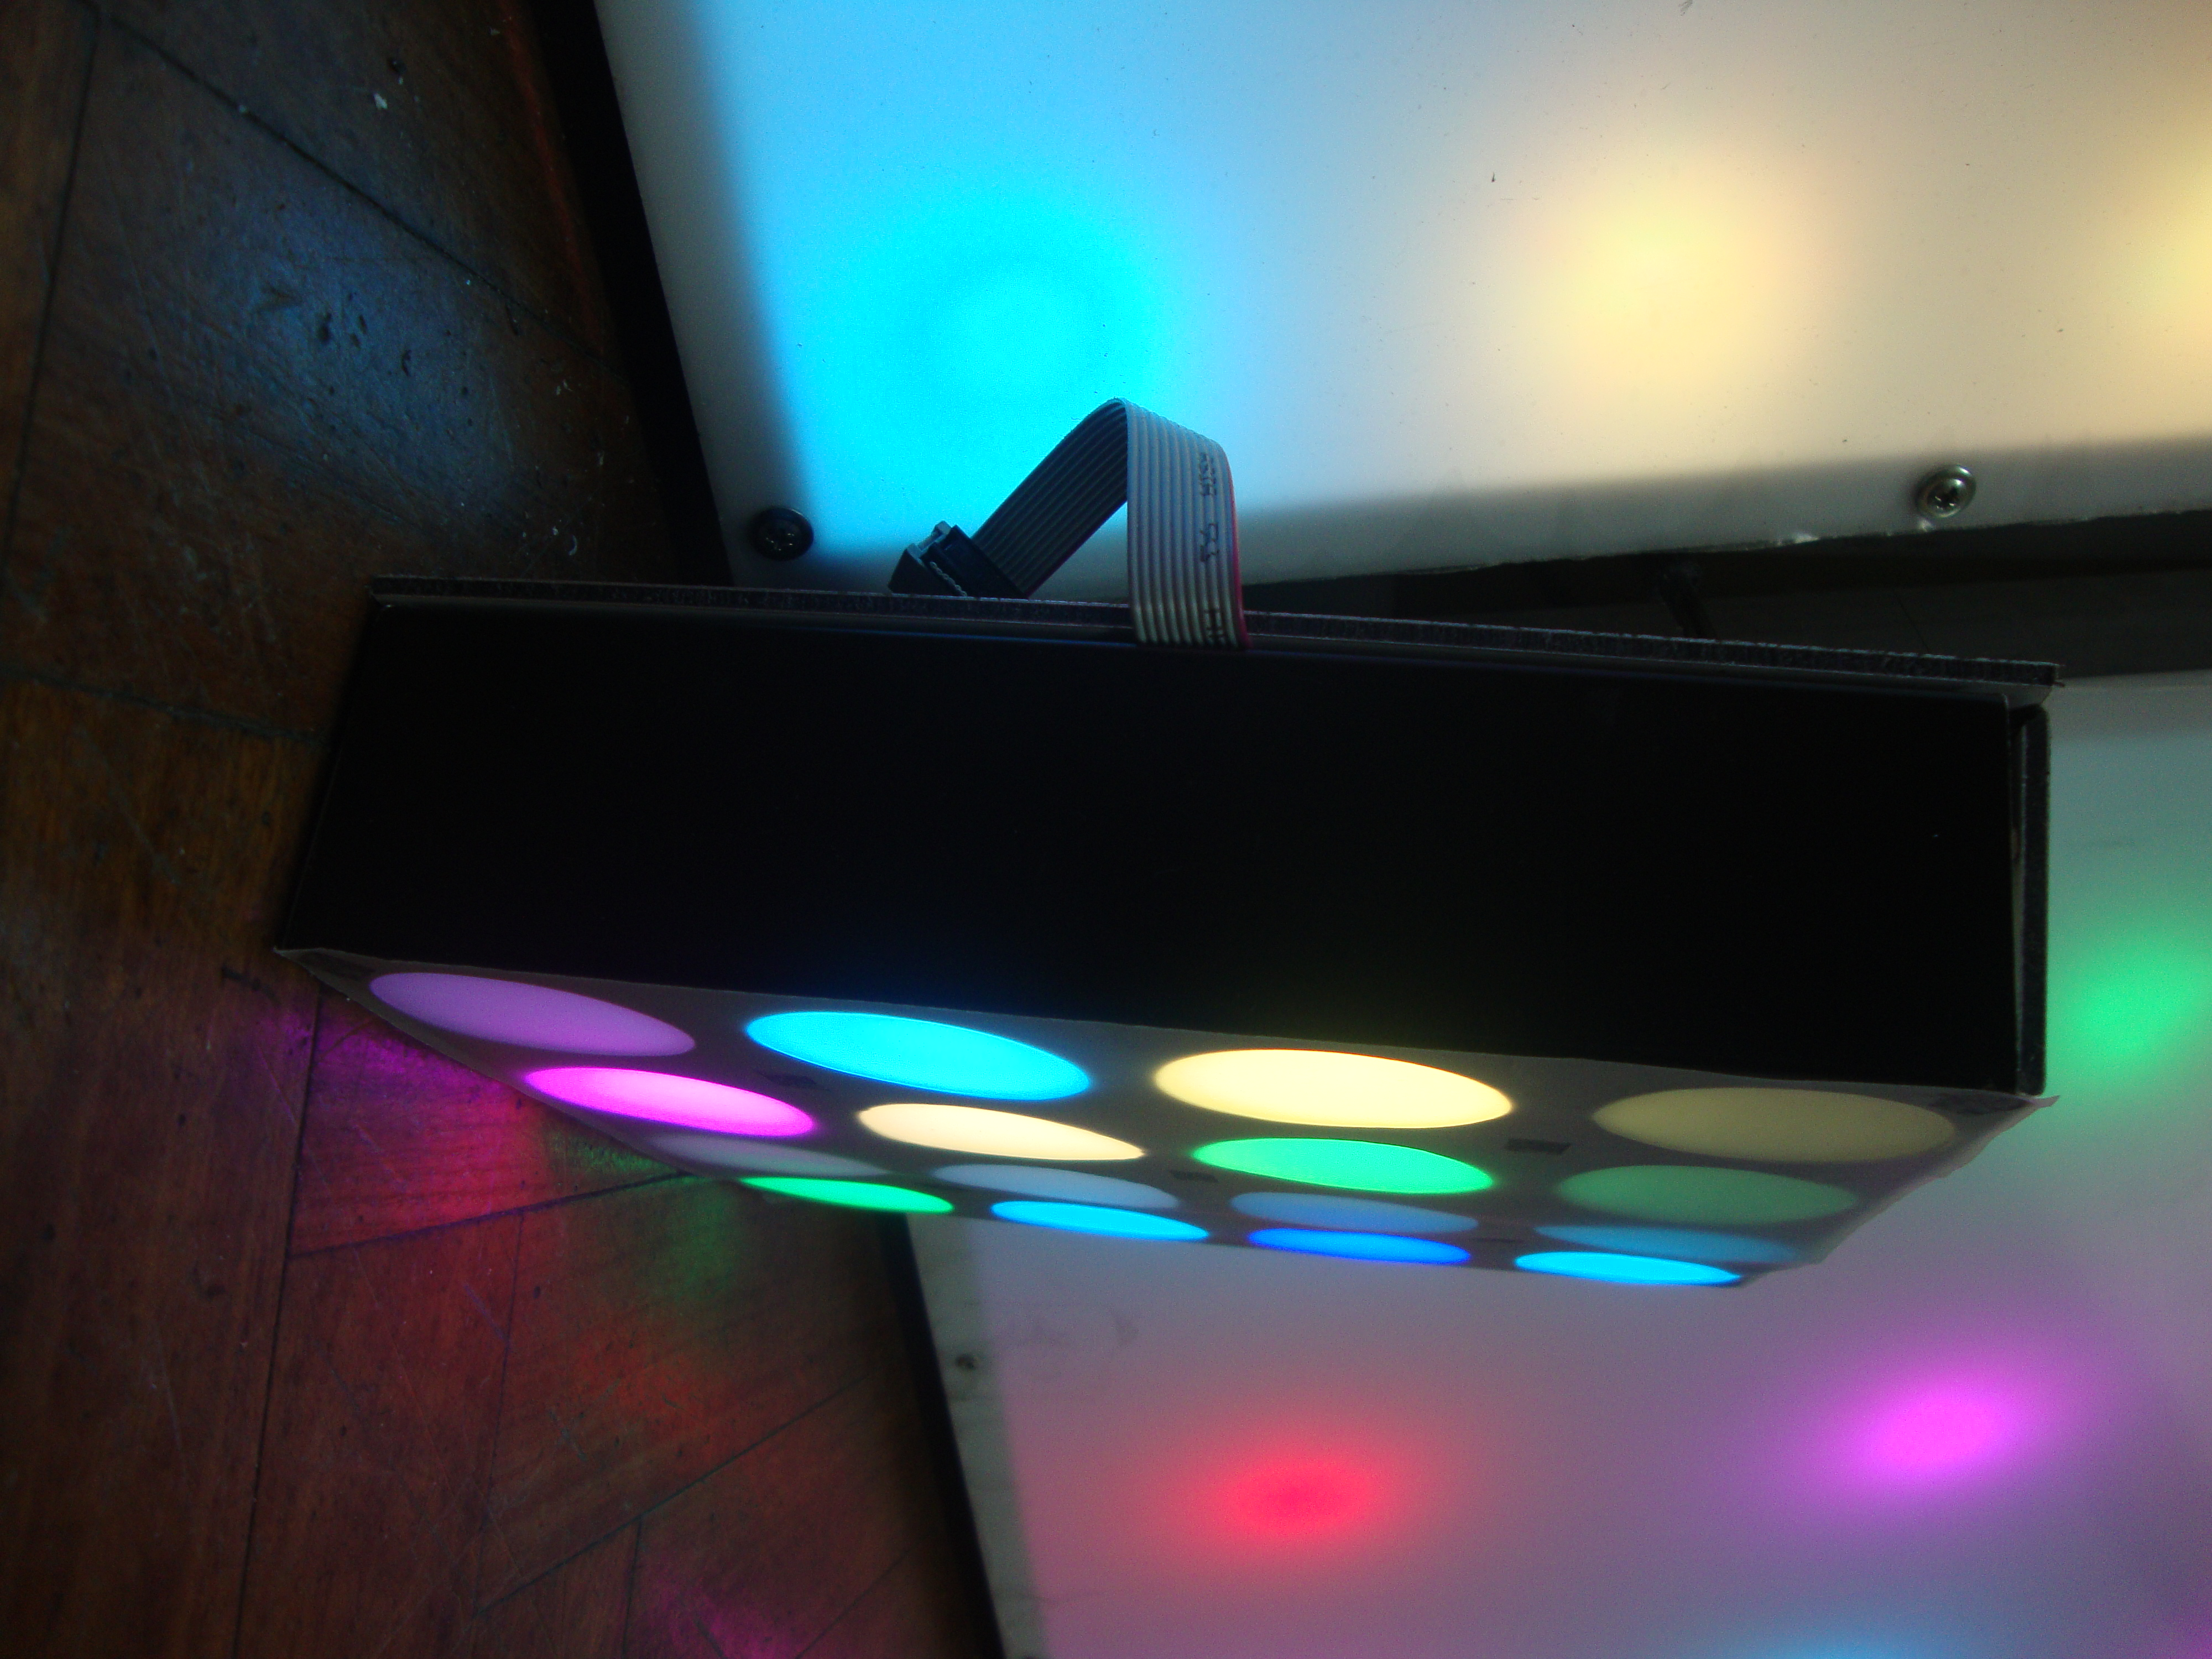
\includegraphics[width=0.24\textwidth]{ledcover4.jpg}
      \end{center}
      \caption{Módulos de leds interconectables para formar pantallas de leds controladas por ethernet de diferentes pitch y tamaños.}
      \label{fig:ledcover}
   \end{figure}

